\documentclass[11pt]{article}
\usepackage{color}
\usepackage{nth}
\usepackage{enumitem}
\usepackage{booktabs}
\usepackage{tabularx}
\usepackage[none]{hyphenat}
\usepackage{hyperref}
\usepackage[pdftex]{graphicx}
\pagestyle{empty}
\setcounter{secnumdepth}{2}
\usepackage{float}

\topmargin=0cm
\oddsidemargin=0cm
\textheight=22.0cm
\textwidth=17cm
\parindent=0cm
\parskip=0.15cm
\topskip=0truecm
\raggedbottom
\abovedisplayskip=3mm
\belowdisplayskip=3mm
\abovedisplayshortskip=0mm
\belowdisplayshortskip=2mm
\normalbaselineskip=12pt
\normalbaselines

% use case stuff
\newcounter{use case ID}

% environment slightly edited from https://tex.stackexchange.com/questions/10293/latex-template-for-use-cases
\newcommand\tabularhead[1]{
    \begin{table}[ht]
        \addtocounter{use case ID}{1}
        \caption{Use Case \arabic{use case ID} - #1}
        \vspace{0.2cm}
        \begin{tabular}{|p{0.2\linewidth}|p{0.70\linewidth}|}
            \hline
            \textbf{Action} & \textbf{#1} \\
            \hline}

        \newcommand\addrow[2]{#1 & #2\\ \hline}

            \newcommand\addmulrow[2]{ \begin{minipage}[t][][t]{2.5cm}#1\end{minipage}
                &\begin{minipage}[t][][t]{11cm}
                    \begin{enumerate}[itemsep=-1ex] #2   \end{enumerate}
                \end{minipage}\vfill\\ \hline}

            \newenvironment{usecase}{\tabularhead}
        {\hline\end{tabular}\end{table}}



        % cheaty non-functional requirement env

        \newcounter{req ID}
        \newcommand\tabularheadfsd[1]{
            \begin{table}[ht]
                \addtocounter{req ID}{1}
                \caption{Non-Functional Requirement \arabic{req ID} - #1}
                \vspace{0.2cm}
                \begin{tabular}{|p{0.2\linewidth}|p{0.70\linewidth}|}
                    \hline
                    \textbf{Action} & \textbf{#1} \\
                    \hline}

                \newenvironment{requirement}{\tabularheadfsd}
                {\hline\end{tabular}\end{table}}

                \begin{document}

                \vspace*{0.5in}
                \centerline{\bf\Large COMP 354}
                \centerline{\bf\Large Requirements for the project myMoney}

                \vspace*{0.5in}
                \centerline{\bf\Large Team PA-PK}

                \vspace*{0.5in}
                \centerline{\today}

                \vspace*{1.5in}
                \begin{table}[htbp]
                    \caption{Team}
                    \begin{center}
                        \begin{tabular}{|r | c|}
                            \hline
                            Name & ID Number \\
                            \hline\hline
                            Anne-Laure Ehresmann & 27858906 \\
                            \hline
                            Marc-Antoine Dube & 40029307 \\
                            \hline
                            Kadeem Caines & 26343600 \\
                            \hline
                            Abdel Rahman Jawhar & 27192142 \\
                            \hline
                            Keith Dion & 40036340 \\
                            \hline
                            Hrachya Hakobyan & 40041555 \\
                            \hline
                            Andrew-Smith & 40034936 \\
                            \hline
                            Dongyu Chen & 27241909 \\
                            \hline
                            Yauheni Karaniuk & 40005680 \\
                            \hline
                            Renny Xu & 40005262\\
                            \hline
                            Wei Wang & 40041116 \\
                            \hline
                        \end{tabular}
                    \end{center}
                \end{table}

                \begin{table}[htbp]
                    \caption{Revision history}
                    \begin{center}
                        \begin{tabular}{|r | c| c |}
                            \hline
                            Version & Date & Changes \\
                            \hline
                            1.1 & \nth{12} March 2018 & fixed business rules\\
                            1.0 & \nth{11} February 2018 & completed requirements \\
                            \hline
                        \end{tabular}
                    \end{center}
                \end{table}


                \tableofcontents
\listoffigures
\clearpage
\listoftables

\clearpage


\section{Document Purpose}

The purpose of this document is to define requirements for the  desktop application myMoney. This document may thus be used to orient the development of the application. It seeks to understand the requirements of the problem, formulate the necessary functions and properties needed to answer this problem and its requirements, and then test these functions against the requirements. Hence, it may be used by our users to specify the problem and its requirements, by the developers to understand what functions their system must implement, and what to test their system against. The primary audience for this document are the stakeholders of the project and the development team of the system, as well the project testers for fine-tuning their testing strategy.

\section{Project description}

\subsection{Problem Introduction}
At the present time, users who have more than one bank account can quickly get overwhelmed with the differing methods of access and interfaces for each account. It becomes arduous to access every account and difficult to visualise how much money one has and how one's budget changes on a day-to-day basis. There exists a plethora of software for money management, each greatly varying in design due to the complex and multifarious clientele. Unfortunately, the high quality programs in this domain also tend to have complex and highly extensive accounting capabilities, and setting them up as well as learning how to use them requires investing some number of hours that often scare off casual users. This lack of appropriate software for simple money management costs time and frustration for the common user, and discourages them from fully taking advantage of services that are provided by their banks, for fear of the complexity that may come with such services. Even simply keeping track of their finances becomes a daunting task, which negatively impacts both the users and the banks. We seek to design a desktop application to solve the most common issues in a simple and lightweight manner. a more in-depth discussion of the user profile is available in section \ref{actors}.

\subsection{System Context}

Our system will mainly involve the user interacting with a desktop application interface. The user shall provide information about his bank accounts to the interface, which the system will store it in a local database. The system then establishes a connection to the banks, passing along the user information. It will receive the data associated with the bank account(s) of the user, which it will then display to the user. Section \ref{func req} gives a more detailed view of all of the functions that the system will be able to perform.

\clearpage

\begin{figure}[htbp]
    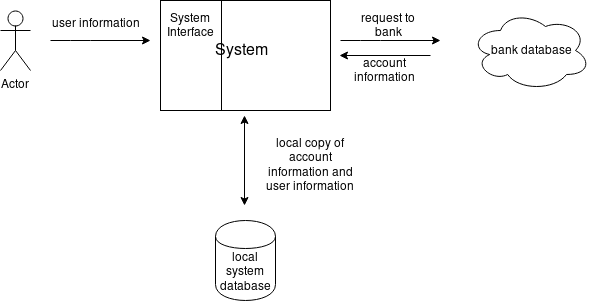
\includegraphics[width=\linewidth]{context.png}
    \caption{System Context}
    \label{fig:system-context}
\end{figure}

\subsection{Project Scope}
myMoney aims to be a small, simple tool which provides an easy method of viewing accounts across multiple banks, their transactions, and categorisation tools for grouping transactions across multiple accounts. One user may create a personal account and link their bank accounts to easily access them through myMoney. They may check the transactions of a specific bank account or all of their bank accounts at once. They may also sort their transactions by date, type, or any other property of the transaction, and categorise certain transactions for better organisation and minimal budgeting. myMoney is intended to work alongside banking institutions: it relies on the data provided by banks to create a transaction history for the users. In short, it seeks to be an application for managing expenses so as to quickly make judgment calls on financial decisions, in a way that is accessible to even the most financially or technologically inexperienced user.

\clearpage

\subsection{Business Goals}

\begin{itemize}
    \item \textbf{Compete with existing solutions}

        We are not the sole developers of budgeting applications by far. Not just that, but users already have a procedure for accessing their bank accounts directly through interfaces provided by banks. As such, if we want to attract users to our product, we must be able to compete on the same playing field as these current applications/procedures. We must, at the very least, meet their level of performance, ease of use, security, and other qualities described in \ref{nonfunc req} for our system.

    \item \textbf{Target market: wide user-base composed mainly of millennials, students, new professionals}

        Our customer group user group and development team happen to involve the same people: young professionals and students with little to no expected background in financing. As customers, this group has no interest in complex budgeting functions (if they do, they are not the target audience aimed by this system), but instead seeks some way of organising tracking their total assets. This group favours lightning-fast applications for frequent yet momentary usage. They want to monitor their cash spending and make long-term financial decisions based on clear, understandable data that they can access and modify rapidly.

    \item \textbf{Future-proof, long-term robustness of the system} We wish to be able to support this system on a long-term basis. We also want to support users who might have a rather long transactional history, or might, over the years of using our application, gain such a transactional history, and these should be accommodated by the system to guarantee long-term success.

    \item \textbf{Reduce total cost of ownership}

        For the above business goal, it is imperative for our application to be relatively cheap to maintain and support after development, as it would lengthen the lifetime of our system.

\end{itemize}

\subsection{Domain Concepts}

\subsubsection{Domain Model}

In this section we provide the domain model of our system, useful for users and documenters seeking to understand the general setup of our system. Useful to understanding this model is the the context of this system, provided in figure \ref{fig:system-context}, to see the connections between the system and the actors.

\begin{figure}[H]
    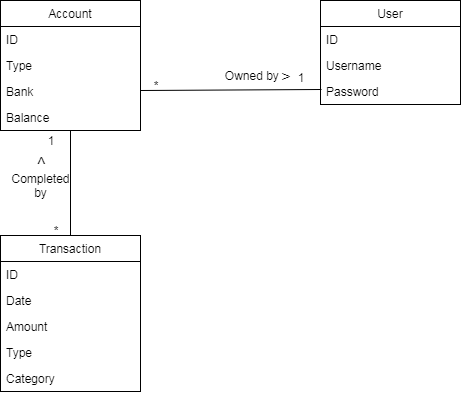
\includegraphics[scale = 1]{DomainModel.png}
    \centering
    \caption{Domain Model}
    \label{fig:domain-model}
\end{figure}

\clearpage


\subsection{Actors} \label{actors}
\subsubsection{User}
Our main actor is the user. All use cases are triggered by the user, as their requests that directly cause the bank system or our system to take action. All identification needed to access the bank system will be provided by the user. Using this information, the system will be able to answer queries made by the user as described in the use cases.
\subsubsection{Bank}
Our sole other actor is the bank(s) system. Each bank system provides an API for accessing its bank account data. Our system will pull this data directly from the bank systems (who act as secondary actors), using identification as given by the user for the bank's authentication system. In other words, our system will merely act as a middleman between the user demanding information in a specific format, and the banks holding that information in an inconvenient format.


\section{Requirements and Business Rules} \label{nonfunc req}
% type: quality, quality goals, quality of service, constraint
\subsection{Non-Functional Requirements}
\begin{requirement}{Reliability and usability}
    \addrow{Requirement ID:}{01}
    \addrow{Type:}{Quality of service}
    \addrow{Description:}{We want to guarantee that our system's reliability is only constrained by the reliability of the bank servers. We also to ensure the application is always usable, except during maintenance or communication with the database.}
    \addrow{Reasoning:}{The current procedure which users employ benefits from near-perfect up-time, as its only constraint is the reliability of the bank servers. In order to be competitive with this current solution, we must match this level of reliability.}
    \addrow{Quality attribute scenario:}{System operates mostly offline, and can function even without access to the internet using past data. System meets security and connectivity performance of current procedure.}
\end{requirement}

\begin{requirement}{Simplicity and ease-of-use}
    \addrow{Requirement ID:}{02}
    \addrow{Type:}{Quality of service}
    \addrow{Description:}{The system should be easy to understand and not overburdened by unused features, allowing for clear display of relevant information.}
    \addrow{Reasoning:}{The current procedure for users to view their bank transactions across different accounts requires them to log in each individual bank account interface, then compare each distinct format for the bank accounts manually. This is tedious for most users, and hence easy to outperform and become competitive with the current procedures. It is also in our interest to pursue this, as our business targets a more casual user-base which tend to favours a simpler and more lightweight application.}
    \addrow{Quality attribute scenario:}{Installation of the system should be easy and require very little, if any, decisions from the user beyond choosing to install the system. With no training, a user should be able to intuitively learn and use the system in a short amount of time.}
\end{requirement}

\begin{requirement}{Performance}
    \addrow{Requirement ID:}{02}
    \addrow{Type:}{Quality of service}
    \addrow{Description:}{The system should ensure minimal load times, notably when connecting to the bank and the local database.}
    \addrow{Reasoning:}{With our target audience in mind, we want to be able to provide adequate performance when the system is used in frequent, short-time bursts. These sorts of applications tend to be popular with millennial audiences. Focusing on performance also renders our system more competitive, as our target audience highly favours quick interactions with the interface.}
    \addrow{Quality attribute scenario:}{System files should be small, less than 50MB. When the system connects to the internet (with reasonable bandwidth) to fetch transactions, they are returned to the user in less than 2 seconds.}
\end{requirement}

%and hence to the shifting the user requirements which may change as our target audience change their demands over time.

\begin{requirement}{Maintainability and testability}
    \addrow{Requirement ID:}{03}
    \addrow{Type:}{Quality}
    \addrow{Description:}{The system should be maintainable on a long-term basis,  A testing suite is imperative for adaptive development, as it aids in reducing time and cost of debugging, and lets us quickly conduct system diagnostics.}
    \addrow{Reasoning:}{Due to the dependency of the system upon the banks' API, it is necessary that the system should be easy to alter and maintain, and hence be capable of adapting to third-party changes. This both reduces costs of ownership and favours long-term use of the application.}
    \addrow{Quality attribute scenario:}{New modifications to the system should be fully covered by unit tests before another modification is implemented.}
\end{requirement}

\begin{requirement}{Security}
    \addrow{Requirement ID:}{04}
    \addrow{Type:}{Quality}
    \addrow{Description:}{The system should guarantee a level of security, requiring valid credentials in order to access any sensitive information and denying access otherwise.}
    \addrow{Reasoning:}{A user's bank information is incredibly sensitive, and any possible security flaw could cripple the entire system and destroy any sort of trusted relationship that users may have developed with our business. It is thus of utmost importance that any data coming from the banks are accessible solely with proper authentication. Improper security would certainly negatively impact user trust in our business.}
    \addrow{Quality attribute scenario:}{Database should be encrypted, and testing suite should include verification of security measures on the system.}
\end{requirement}

\begin{requirement}{Portability}
    \addrow{Requirement ID:}{05}
    \addrow{Type:}{Quality}
    \addrow{Description:}{Since the system is fairly lightweight, it should also focus on compatibility with older hardware (within reason) and support numerous operating systems, to encourage a wide user-base.}
    \addrow{Reasoning:}{We want to cater to a wide and somewhat casual audience, who may not be technologically adept and still rely on old (but familiar) hardware. The lightweight quality of our application means that it would easily be run on older hardware, provided we also ensure compatibility with said hardware.}
    \addrow{Quality attribute scenario:}{System should support older versions of popular OS's, such as windows 7/windows vista.}
\end{requirement}

\begin{requirement}{Scalability}
    \addrow{Requirement ID:}{06}
    \addrow{Type:}{Quality}
    \addrow{Description:}{The system should function even on a long-term basis, and hence be capable of handling a growing number of transactions. The scaling size of the database should be managed by the system so as not to overwhelm the hardware it is running on.}
    \addrow{Reasoning:}{As we foresee our system being used on a long period of time, we should also acknowledge the possibility of users acquiring a large history of transactions over time. We should thus plan accordingly and put measures of precautions so as not to overwhelm their machines when loading in a large database. Crippling their machine could result in a negative perception of business and system.}
    \addrow{Quality attribute scenario:}{System should use SQLite to minimize database size, and take precautions not to load an entire database in memory should the number of transactions exceed a size that may be unmanageable by the hardware.}
\end{requirement}

\begin{requirement}{Data integrity}
    \addrow{Requirement ID:}{07}
    \addrow{Type:}{Quality}
    \addrow{Description:}{Bank accounts data (description as well as transactions) must match the data provided by the banks.}
    \addrow{Reasoning:}{For obvious reasons, we want to guarantee data integrity. Not meeting this requirement would harm the reputation of the business, and render the system rather useless.}
    \addrow{Quality attribute scenario:}{system should verify data validity, and tests should include verification of matching data between the local database and the banks' database}
\end{requirement}

\begin{requirement}{Java}
    \addrow{Requirement ID:}{08}
    \addrow{Type:}{Design Constraint}
    \addrow{Description:}{The system should be programmed in Java.}
    \addrow{Reasoning:}{To take advantage of the JVM's portability, we would be able to develop for numerous platforms whilst having to maintain a single version of the system.}
\end{requirement}

\begin{requirement}{Object-oriented design}
    \addrow{Requirement ID:}{09}
    \addrow{Type:}{Design Constraint}
    \addrow{Description:}{The design of the system should be object-oriented.}
    \addrow{Reasoning:}{As we will be using java, we should embrace the style of the language and use object-oriented programming. This will also ease maintainability and portability.}
\end{requirement}

    \begin{requirement}{Model-view-controller architecture}
        \addrow{Requirement ID:}{10}
        \addrow{Type:}{Design Constraint}
        \addrow{Description:}{The design of the system should use a MVC architecture.}
        \addrow{Reasoning:}{As our main development time for creating a prototype is fairly short, using MVC will allow us to properly segment each part of our code, and thus give it a strict structure, as well as make it more easily maintainable and testable.}
    \end{requirement}

    \begin{requirement}{SQLite database}
        \addrow{Requirement ID:}{11}
        \addrow{Type:}{Design Constraint}
        \addrow{Description:}{The system should use SQLite}
        \addrow{Reasoning:}{As our system is fairly simple and favours a lightweight design, using a more complex database would be a waste of resources.}
    \end{requirement}

\clearpage

\subsection{Business Rules} \label{biz rules}

These business rules are the limits placed on the functions described in \ref{func req}.

\begin{itemize}
    \item \textbf{BR1: Length on account parameters set by the user}
    \begin{itemize}
        \item All user-set account parameters, such as username or password, must be between 4 and 16 characters long.
        \item \textit{Reasoning:} We do not want usernames and passwords to be too short for security concerns, nor do we want them to be too long, for data size concerns.
    \end{itemize}
\end{itemize}

\begin{itemize}
    \item \textbf{BR2: } User Account authentication
    \begin{itemize}
        \item A user must be correctly authenticated before he may view any data related to a user account, such as user account username and other paramaters, bank accounts associated with said user account, or bank account transactions. To be properly authenticated (also referred to as 'login in'), a user must provide the correct username and password.
        \item \textit{Reasoning:} Privacy is a huge concern for users when dealing with their financial information. Hence, we want to ensure that none of their data may be accessed unless the user has authenticated access to the account in question.
    \end{itemize}
\end{itemize}


\begin{itemize}
    \item \textbf{BR3: }User Account authorisation
    \begin{itemize}
        \item A user may only view or edit information related to the user account he has logged into. He may not view or edit bank accounts or user account information of other users.
        \item \textit{Reasoning:} For privacy concerns once again, we want to ensure that a user may only modify that which he can access through authentication. We clarify the separation between authentication (actually logging in) and authorisation (what level of authority comes with being logged in?).
    \end{itemize}
\end{itemize}


\begin{itemize}
    \item \textbf{BR4: } Bank authorisation
    \begin{itemize}
        \item  A user may only add bank accounts once he has logged in, and he may only add account to which he has authorised access, given to him by his bank. He verifies this by providing the bank account ID of the bank account he wishes to access.
        \item \textit{Reasoning:} We want to ensure we follow the authentication requirements of the banks, once again for privacy reasons, but also to ensure a good-faith relationship with the banks is kept.
    \end{itemize}
\end{itemize}




\subsection{Functional Requirements} \label{func req}

This section will cover the functional requirements associated with the myMoney app. These are the software capabilities that must be present in order for the user to carry out the services provided by the app or to execute the use cases.

\begin{itemize}
    \item  \textbf{User account creation:} The system allows the creation of user accounts, with information (user-name, password, first name, and last name) provided by the user.
    \item \textbf{User account authentication:} The system shall grant a user access only to a properly authenticated user. If a user does not enter credentials, the system shall notify the user of the failure to authenticate.
    \item \textbf{User account management:} The system shall require proper authentication to modify and/or delete a user account.
    \item  \textbf{Bank account management:} The system permits a logged-in user to add, manipulate, or remove bank accounts that are connected to the user account.
    \item  \textbf{Transaction management:} The system permits a logged-in user to access the details of transactions associated with all bank accounts that were added to the user account. The system obtains these transactions through the banking system's API. The system allows different display formats, such as 'sorted by date' or 'sorted by type' or 'sorted by bank account.
    \item \textbf{Categorisation:} The system permits the categorisation of transactions, a property by which the transactions may be sorted.
\end{itemize}

\section{User-Stories}

\textbf{User-Story 1}

As a user, I should be able to create, manage and delete my user account. I should have the options to view and update personal information to facilitate more efficient use of the application and personalise my experience.

\textit{Acceptance criteria:}
\begin{itemize}
    \item It should possible to sign up with a username and a password.
    \item It should be possible to update personal information, including the name, email address, phone number and password.
    \item The application should provide quality user experience when accessing and updating account information
\end{itemize}

\clearpage

\textbf{User-Story 2}

As a user, I should have ability to manage my bank account information. The application should allow me to connect my bank accounts, remove bank accounts and view all the information associated with the bank account.

\textit{Acceptance criteria:}
\begin{itemize}
    \item It should be possible to connect a bank account to the application.
    \item It should be possible to remove a bank account from the application.
    \item The application should display bank account information including:
        \begin{itemize}
            \item Bank account ID
            \item  Bank name
            \item Account type
            \item Account balance
            \item History of transactions
        \end{itemize}
    \item The application should provide a way to see bank account statements for a specific period.
    \item It should be possible to sort the list of all bank account transactions by any of its attributes, such as the type of the transaction and the amount.
\end{itemize}

\textbf{User-Story 3}

As a user, I should have the ability to group my bank account transactions into categories, to be able to manage my finances more efficiently.

\textit{Acceptance criteria:}
\begin{itemize}
    \item The application should allow to assign a transaction to a category, such as monthly payments, groceries, leisure, etc.
    \item I should be able to view transactions of a particular category.
\end{itemize}

\subsection{Description of File Format: Input}

The user enters plain text through the interface of the system. The banking systems provide bank account data by passing a copy of their account, in binary form.

\subsection{Description of File Format: Output}

The system outputs its database data in plain text form, displayed through its interface.

\section{Glossary of Domain Concepts} \label{glossary}
\begin{table}[H]
    \caption{Glossary of Domain Concepts}
    \begin{center}
        \scalebox{0.7}{
            \begin{tabular}{|l|p{0.8\linewidth}|}
                \hline
                Expression &  Definition \\
                \hline
                User & The person that is using the application and the main provider of requests to the system. \\
                \hline
                User Account & A data object containing user information. It also contains the various bank accounts that a user may have linked to the system. \\
                \hline
                Bank Account & A data object containing transactions linked with a specific bank account in a bank institution. One user account may have more than one bank accounts.\\
                \hline
                Transaction & Any kind of money exchange associated with a bank account.\\
                \hline
                Transfer & A type of transaction that occurs between two parties.\\
                \hline
                Deposit & A type of transaction where the owner puts money in his own bank account.\\
                \hline
                Withdrawal & A type of transaction where the owner of the bank account removes money from his balance.\\
                \hline
                Database & A local or online container which holds data in an organised, efficient manner. \\
                \hline
                Server & a computer that is accessible on a network, on which a database and/or system may be hosted. The bank institutions' databases will be hosted on here. \\
                \hline
                Object-Oriented Programming & A programming paradigm which separates entities into objects, and uses the concept of inheritance of properties, polymorphism of objects, encapsulation of objects. We use this paradigm for its maintainability and structural benefits.\\
                \hline
                MVC - Model-View-Controller Architecture & An architectural pattern which strictly separates components into the model (manages the data and logic), the view (output of the model), and the controller (handling input and passing it to the model or view).\\
                \hline
                Interface & A component of a system by which other entities (be it humans or other systems) may engage in an exchange of data with the system in question. \\
                \hline
                API - Application Programming Interface & A protocol or set of functions which serve as a method of communication to a software system. It is a type of interface, and the one by which our system will communicate with the banking institutions' databases. \\
                \hline
                DAO - Data access object & An object that provides an abstract interface to some type of database or other persistence mechanism.\\
                \hline

            \end{tabular}}
    \end{center}
\end{table}

\clearpage


\section{Use Cases}
\subsection{Overview}
Use cases 1 through 4 deal with the user manipulating his accounts. Use cases 5 through 7 and 9 deal with the user viewing the data in different formats. Use case 8 deals with the user manipulating the transactions' formats. For iteration 1, we have only included use case 1, 3, 5, and 6, as those are the ones we have fully implemented. Below is figure \ref{fig:use-case-diagram} which represents our use case diagram. Following this diagram, we list our uses cases

\begin{figure}[htbp]
    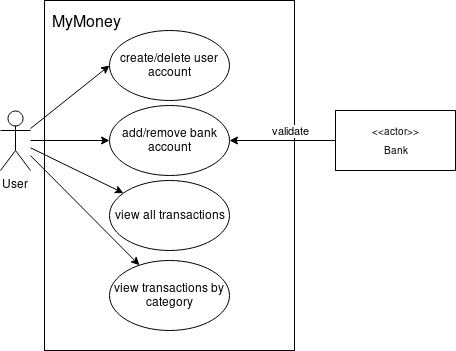
\includegraphics{UseCaseDiagram.png}
    \caption{Use Case Diagram}
    \label{fig:use-case-diagram}
\end{figure}

\begin{usecase}{Create User Account}
    \addrow{Case ID}{01}
    \addrow{Summary}{User gives information about a new user account, system validates it and creates the account.}
    \addrow{Description} {This use case describes how a user can create their own account for the myMoney application in order to use the application, add bank accounts and view and categorize their transactions}
    \addrow{Scope}{money and budget management application}
    \addrow{Level}{user-goal}
    \addrow{Actors}{\textbf{User}}
    \addmulrow{Stakeholders and Interests}{
    \item User: Wants fast and easy account creation, clear and comprehensible display, proof of successful account creation.
    \item Company: Wants user interests to be fulfilled, wants to prevent erroneous input, wants fast communication with the local account database as well as fault tolerance in case of database conflicts, issues with editing authorization, or other possible database problems.}
    \addrow{Pre-Conditions}{User has opened the application and is in the sign-up menu.}
    \addrow{Success Guarantee}{Account successfully saved in local account database, with name and password as specified by the user.}
    \addmulrow{Main Success Flow}{
    \item User enters a user-name, first name, last name, and password.
    \item System validates user-name and password
    \item System creates new account.
    \item System notifies the user of the successful account creation}
    \addmulrow{Exceptions}{
    \item User account is not created if there is an existing user name
    \item Account is not created if password does not match specified format}
    \addrow{Post-Conditions}{The application will return the user to the home menu after a successful account creation. User can then log into the system  }
    \addrow{Priority}{High}
    \addrow{Traces to Test Cases}{}
\end{usecase}

\begin{usecase}{Delete User Account}
    \addrow{Case ID}{02}
    \addrow{Summary}{User deletes a user account from the local accounts database, removing all bank accounts and information associated with that account.}
     \addrow{Scope}{money and budget management application}
     \addrow{Level}{user-goal}
     \addrow{Actors}{\textbf{User}}
     \addmulrow{Stakeholders and Interests}{
     \item User: Wants easy navigation and secure account deletion, no risk of accidental deletion, proof of successful account deletion.
     \item Company: Wants user interests to be fulfilled, wants to ensure clean deletion from the database. }
     \addrow{Pre-Conditions}{User has logged in the user account he wants to delete.}
     \addrow{Success Guarantee}{user account is successfully deleted, all associated bank information is deleted, and user is returned to the home menu.}
     \addmulrow{Main Success Flow}{
     \item User enters the account settings, then selects 'delete account'.
     \item System brings up a confirmation menu to ensure that this selection was not accidentally entered.
     \item User confirms his choice.
     \item System successfully deletes all relevant entries in the local database, then notifies the user of this successful deletion.
     \item User confirms having read this notification.
     \item System brings the user back to the home menu.}
     \addrow{Exceptions}{}
     \addrow{Post-Conditions}{}
     \addrow{Priority}{}
     \addrow{Traces to Test Cases}{}
\end{usecase}


\begin{usecase}{Add Bank Account to a User Account}
    \addrow{Case ID}{03}
    \addrow{Summary}{User gives information about a new bank account, system sends it to the bank for verification then creates necessary entries in the local database once the bank approves the information.}
    \addrow{Scope}{money and budget management application}
    \addrow{Level}{user-goal}
    \addrow{Actors}{\textbf{User}, Bank}
    \addmulrow{Stakeholders and Interests}{
    \item User: Wants fast and easy account creation, clear and comprehensible display, proof of successful account creation.
    \item Company: Wants user interests to be fulfilled, wants to prevent erroneous input, wants fast communication with the local account database as well as the bank, wants fault tolerance in case of database conflicts, issues with the bank, or other possible local database problems.
    \item Bank: Wants to satisfy its customer base, wants correctly formatted account information given to its API, inexpensive and non-redundant communication of bank account data to third-party applications.}
    \addrow{Pre-Conditions}{User has logged in a user account and is in the user home menu.}
    \addrow{Success Guarantee}{Bank account successfully saved in local account database, with information corresponding the data validated by the bank.}
    \addmulrow{Main Success Flow}{
    \item User enters his/her bank account number.
    \item System validates input, and sends it to the bank for verification and connection.
    \item Bank validates bank account number, and then responds with the bank account information.
    \item System records the valid bank account details securely in its database, and notifies the user of the successful addition of the bank account in the database.}
    \addmulrow{Exceptions}{
        \item Account is not added if an invalid account ID was provided
        \item Account is not added if the account has already been added
        \item Account is not added if an account could not be found by the bank}
    \addmulrow{Post-Conditions}{
        \item The account has been added. Account displayed in account list.
        \item The account has not been added. An error will be displayed describing what went wrong}
    \addrow{Priority}{High}
    \addrow{Traces to Test Cases}{}
\end{usecase}

\begin{usecase}{Remove Bank Account from a User Account}
    \addrow{Case ID}{04}
    \addrow{Summary}{User deletes a bank account from the local database.}
     \addrow{Scope}{money and budget management application}
     \addrow{Level}{user-goal}
     \addrow{Actors}{\textbf{User}}
     \addmulrow{Stakeholders and Interests}{
     \item User: Wants easy navigation and secure account deletion, no risk of accidental deletion, proof of successful account deletion.
     \item Company: Wants user interests to be fulfilled, wants to ensure clean deletion from the database. }
     \addrow{Pre-Conditions}{User has logged in the user account whose active association with a bank account is the one the user wants to delete.}
     \addrow{Success Guarantee}{Bank account is successfully removed from that user account, all associated bank information is deleted from the local database, and user is returned to the account home menu.}
     \addmulrow{Main Success Flow}{
     \item User selects the account he wants to remove, then selects 'remove account'.
     \item System brings up a confirmation menu to ensure that this selection was not accidentally entered.
     \item User confirms his choice.
     \item System successfully deletes all relevant entries in the local database, then notifies the user of this successful deletion.
     \item User confirms having read this notification.
     \item System brings the user back to the home account menu.}
     \addrow{Exceptions}{}
     \addrow{Post-Conditions}{}
     \addrow{Priority}{}
     \addrow{Traces to Test Cases}{}
\end{usecase}

\begin{usecase}{View Transactions for Specific Bank Account}
    \addrow{Case ID}{05}
    \addrow{Summary}{User selects specific bank account and views transactions associated with with selected bank account}
    \addrow{Scope}{money and budget management application}
    \addrow{Level}{user-goal}
    \addrow{Actors}{\textbf{User}}
    \addmulrow{Stakeholders and Interests}{
    \item User: Wants quick and convenient viewing of previous transactions from one specific bank account
    \item Company: Wants to give user ability to micromanage every aspect of the application down to each bank account and transaction.}
    \addrow{Pre-Conditions}{User has created and logged into a user account, and has added at least one bank account to his/her myMoney account. }
    \addrow{Success Guarantee}{User can view transaction by bank account.}
    \addmulrow{Main Success Flow}{
    \item User selects specific bank account from list of all accounts.
    \item System displays all previous transactions under specified bank account.
    \item User selects desired transaction.
    \item System shows all information about desired transaction, such as date and amount withdrawn, deposited, or transferred.}
    \addrow{Exceptions}{}
    \addrow{Post-Conditions}{}
    \addrow{Priority}{}
    \addrow{Traces to Test Cases}{}
\end{usecase}

\begin{usecase}{View All Transactions from all Bank Accounts}
    \addrow{Case ID}{06}
    \addrow{Summary}{User can view all transactions that have been made from all bank accounts}
    \addrow{Scope}{money and budget management application}
    \addrow{Level}{user-goal}
    \addrow{Actors}{\textbf{User}}
    \addmulrow{Stakeholders and Interests}{
    \item User: Wants easy and convenient viewing of all transactions among all bank accounts.
    \item Company: Wants user interests to be fulfilled.}
    \addrow{Pre-Conditions}{User has created and logged into a user account, and at least one bank account has been added to his/her myMoney account.}
    \addrow{Success Guarantee}{User is able to conveniently view all transactions from all institutions in one display.}
    \addmulrow{Main Success Flow}{
    \item User selects View All Transactions option.
    \item System shows all transactions across all accounts on one display.}
    \addmulrow{Exceptions}{
    \item User has not added any account.
    \item User has no any transaction record.}
    \addrow{Post-Conditions}{}
    \addrow{Priority}{High}
    \addrow{Traces to Test Cases}{}
\end{usecase}

\begin{usecase}{Update User Account}
    \addrow{Case ID}{07}
    \addrow{Summary}{User can make changes and update personal information}
    \addrow{Scope}{money and budget management application}
    \addrow{Level}{user-goal}
    \addrow{Actors}{\textbf{User}}
    \addmulrow{Stakeholders and Interests}{
    \item User:  Wants to change personal information to keep up-to-date records on information such as address and email as well as changing user account password.
    \item Company: Wants user interests to be fulfilled. }
    \addrow{Pre-Conditions}{User has created and logged in a user account.}
    \addrow{Success Guarantee}{User can easily update changes in personal information to guarantee accurate personal records }
    \addmulrow{Main Success Flow}{
    \item User selects update user account information.
    \item System shows current user account information.
    \item User selects the piece of information that requires updating.
    \item User enters new information.
    \item System updates and saves the new information.
    }
    \addrow{Exceptions}{}
    \addrow{Post-Conditions}{}
    \addrow{Priority}{}
    \addrow{Traces to Test Cases}{}
\end{usecase}

\begin{usecase}{Categorize Transaction}
    \addrow{Case ID}{08}
    \addrow{Summary}{User can select a category to represent a transaction.}
    \addrow{Description} {This use case describes how a user can categorize their transactions with specific labels in order to sort their spending and better manage where most of their money is being spent }
     \addrow{Scope}{money and budget management application}
     \addrow{Level}{user-goal}
     \addrow{Actors}{\textbf{User}}
     \addmulrow{Stakeholders and Interests}{
     \item User: Wants to label each transaction as a specific type of spending, such as rent, bills, leisure, etc., to better manage and track spending habits.
     \item Company: Wants user interests to be fulfilled. Wants to facilitate user's ability to budget and manage money through simple categorization of spending.}
     \addrow{Pre-Conditions}{User has created and logged in a user account, added at least one bank account, and has made at least one type of transaction.}
     \addrow{Success Guarantee}{User can quickly and efficiently categorize each transaction.}
     \addmulrow{Main Success Flow}{
     \item User selects desired transaction to categorize.
     \item User selects the categorize option.
     \item System displays the categories in a drop down menu.
     \item User selects preferred category to represent the current transaction.
     \item System saves transaction under chosen category.}
     \addmulrow{Exceptions} {
     \item User has not added a bank account and cannot categorize any transactions within until one is added \item User does not have any transactions within his bank account and cannot categorize anything}
     \addrow{Post-Conditions}{User will have organized his transactions into specific categories of his choosing for easier viewing. The application will save these new categorized transactions.}
     \addrow{Priority}{High}
     \addrow{Traces to Test Cases}{}

\end{usecase}

\begin{usecase}{View Transactions by Any Attribute}
    \addrow{Case ID}{09}
    \addrow{Summary}{User can view transaction by any attribute, from date of purchase or amount of purchase to category of purchase or type.}
    \addrow{Scope}{money and budget management application}
    \addrow{Level}{user-goal}
    \addrow{Actors}{\textbf{User}}
    \addmulrow{Stakeholders and Interests}{
    \item User: Wants to view transactions sorted by any one attribute.
    \item Company: Wants to optimize the ease in which a user can allocate his/her budget, and track spending habits.}
    \addrow{Pre-Conditions}{User has created and logged in a user account, has added at least one bank account, and has made at least one transaction.}
    \addrow{Success Guarantee}{User can view categorized transactions by selecting one attribute. Default sorting is ascending order by alphabet or value of number. Click the same attribute twice will sort in descending order.}
    \addmulrow{Main Success Flow}{
    \item User clicks the button<View All Transactions>.
    \item System shows all transactions from all accounts on one display.
    \item User selects to view sorted transaction by clicking any one attribute.
    \item System sorts transactions by the selected attribute in ascending order.}
    \addmulrow{Exceptions}{
    \item User has not added any account.
    \item User has no any transaction record.}
    \addrow{Post-Conditions}{}
    \addrow{Priority}{High}
    \addrow{Traces to Test Cases}{}
\end{usecase}

\clearpage
\section{Reference}

\begin{itemize}
    \item User information: As our user and use-cases was based on feedback provided by our developers, our references lie mainly within our own team.
    \item Craig Larman - Applying UML and Patterns
    \item Greg Butler's course COMP 354 content
    \item \href{http://web.mit.edu/ssit/cis/CISRequirements.html}{\textcolor{blue}{MIT Curricular Information System
        Software Requirements Document}}
    \item \href{https://resources.sei.cmu.edu/asset_files/TechnicalReport/2005_005_001_14621.pdf}{\textcolor{blue}{Carnegie Mellon Business Goals}}
    \item \href{http://www.oracle.com/technetwork/testcontent/gettingstartedwithusecasemodeling-133857.pdf}{\textcolor{blue}{Use-Case: Oracle }}

\end{itemize}
\end{document}
